%Package Float verwendet -> Option [H] erzwingt Platz für Grafik
\mdfsetup{
%
frametitle={
%
\tikz[baseline=(current bounding box.east),
outer sep =0pt]
\node[anchor=east,rectangle,fill=red]
{\color{white} \small Nina \& Oma Lena};},
frametitleaboveskip=\dimexpr-\ht\strutbox\relax
}
\pagenumbering{gobble}
\chapter*{\FontH{\Huge Nina und die rosa Delphine}}
\addcontentsline{toc}{chapter}{Nina und die rosafarbenen Delphine}
\centerline{\Huge \color{red}\SixFlowerPetalDotted}
\vspace{20pt}
\centerline{\bf \Large\color{red}Für Oma Carola zum Geburtstag }
\vspace{20pt}
\centerline{\bf \Large\color{red} von Linda und Gordon}
\vspace{20pt}
\centerline{\huge \color{red}\SixFlowerPetalDotted}
\vspace{20pt}
\centerline{\LARGE \color{red}\SixFlowerPetalDotted}
\vspace{20pt}
\centerline{\Large \color{red}\SixFlowerPetalDotted}
\vspace{20pt}
\centerline{\large \color{red}\SixFlowerPetalDotted}
\vspace{20pt}
\centerline{\normalsize \color{red}\SixFlowerPetalDotted}
\vspace{20pt}
\centerline{\small \color{red}\SixFlowerPetalDotted}
\vspace{20pt}
\centerline{\footnotesize \color{red}\SixFlowerPetalDotted}
\vspace{20pt}
\centerline{\scriptsize \color{red}\SixFlowerPetalDotted}
\vspace{20pt}
\centerline{\tiny \color{red}\SixFlowerPetalDotted}
\newpage
\pagenumbering{arabic}
\begin{mdframed}[style=mystyle]
\lettrine[lines=3]{\color{red}H}{eute} war Oma Lena zu Besuch. Nina hatte sich schon lange auf sie gefreut. Oma Lena wohnte leider weit weg, in einem anderen Land und deswegen konnten sich die beiden nicht so oft sehen. Aber jetzt war es wieder so weit. 

Es war schon spät geworden, Geschenke mussten ja noch ausgepackt werden und dann Abendessen. Nina fand, dass Erwachsene immer viel zu viel Zeit mit Essen vergeuden. Anstatt stundenlang am Tisch zu sitzen, könnte man die Zeit doch viel besser nutzen. Sie würde das später, wenn sie gross sein wird, anders machen, so viel war klar.

\enquote{Also gut} rief der Papa aus der Küche, \enquote{Oma darf dir noch eine Geschichte vorlesen. Aber nicht mehr so lange. Eine Viertelstunde, höchstens! Morgen ist wieder Kindergarten und dann musst du fit sein Nina.}

Nina seufzte. Als ob das jetzt wichtig wäre, dass sie morgen früh aufstehen muss. 

\enquote{Ist doch mir egal.} brummte sie und streckte die Zunge raus, aber so, dass Papa das nicht sehen konnte. Oma Lena hatte ein Buch mitgebracht, das war das Geschenk gewesen. Eins von rosafarbenen Delphinen. Mama meinte, dass es die wirklich gäbe. Weit weg in einem Fluss namens Amazonas, der mitten durch einen Urwald fliesst. Nochmals schnell auf der Karte nachsehen, wo der eigentlich liegt.

Nach dem Zähneputzen konnte Nina endlich ins Bett springen und auf Oma warten. Nina überlegte, ob Mama ihr manchmal extra lange die Zähne putzte, um sie zu ärgern. Man könnte schon manchmal den Eindruck haben. Kater Fritz war auch gekommen, das war so seine Gewohnheit. Er sprang auf die Decke von Nina und wollte wohl auch zuhören. Fritz und Nina waren gute Freunde, obwohl er manchmal alleine mit Ninas Sachen spielte und die dann weg waren. Manchmal dauerte es Tage, bis die Sachen in irgendeiner Ecke wieder auftauchten. 

Oma setzte sich auf die Bettkante, klappte das Buch auf und blätterte ein bisschen zwischen den Seiten.

\enquote{Bis hierhin lese ich Dir heute vor, den Rest dann morgen. Einverstanden?} Oma tippte dazu auf eine Seite mit dem Bild eines Delphins. 

\enquote{Naaa gut.} antwortete Nina. Was sollte sie auch machen? Und erst einmal anfangen, der Rest findet sich später von alleine.
\end{mdframed}\medskip

Der Urwald ist für gewöhnlich ein ziemlich lauter Ort. Es scheint, dass alle Tiere noch lauter sein wollen, als die anderen. An einem Nebenarm des Amazonas war es diesmal besonders laut, denn es wurde ein grosses Fest gefeiert. Die Regenzeit, die grosse Teile des Urwaldes unter Wasser gesetzt hatte, war so langsam vorbei, nur gelegentlich gab es noch einen Sturm. 

Ein Lied war zu hören.

\enquote{\it feliz cumpleanos a ti, 

feliz cumpleanos a ti

que los cumplas muy feliz

feliz cumpleanos a ti}

Das ist {\it Happy Birthday to you} auf Spanisch. Am Amzonas wird nämlich auch Spanisch gesprochen und heute hatte Rosa Geburtstag. Den Fünften. Rosa war ein Delphinkind, das in einem Nebenfluss eben jenes Amazonas lebte. Die Bäume am Rande des Flusses waren festlich geschmückt. Papageien hatten bunte Federn aufgehängt, das war ein herrlicher Anblick zusammen mit den Schmetterlinge, die überall durch die Luft schwirrten. Ein Ameisenbär steckte seinen Rüssel ins Wasser und machte Blasen, dass es nur so spritzte. Selbst das Faultier drehte seinen Kopf, um zu sehen, was da los ist. Und das musste was bedeuten, Rosa konnte sich nicht erinnern, überhaupt schon einmal gesehen zu haben, dass sich das Faultier bewegt hatte.

Rosas Geburtstag war ein grosses Ereignis. Der fünfte Geburtstag ist nämlich bei Delphinen etwas ganz besonderes. Dann dürfen sie zum ersten Mal alleine aus dem Nebenfluss in den riesigen Amazonas schwimmen. Es ist Tradition, dass sie dann mindestens einen Tag alleine im Amazonas sind. Wer das schafft, ist erwachsen. Ausser Mama und Papa müssen die anderen Delphine dann \enquote{Sie} zu einem sagen. Weil Delphine nicht so alt werden wie wir Menschen, ist es bei ihnen schon mit fünf soweit. Aber ganz ausgewachsen sind sie dann auch noch nicht.

Der erste eigene Ausflug ist immer etwas besonderes. Aufpassen, heisst es dann, denn es gibt viele Gefahren. Am gefährlichsten sind die Alligatoren. Wenn man da als kleiner Delphin nicht aufpasst, macht es Schnapp und weg ist man. Aber fünfjährige Delphine sind so gute Schwimmer, dass das eigentlich nie passiert. Auch vor Zitterallen muss man sich hüten. Wenn man die berührt, versetzen sie einem einen Stromschlag, der sehr weh tun kann. Onkel Konrad war das mal passiert, tagelang hatte er gejammert.

Rosa hatte natürlich ihre vier besten Freunde eingeladen. Es gab Fischkuchen, so wie ihn nur die Oma backen konnte. Rosas Freunde waren auch schon alle fünf, sie war die letzte. Sie hatten sich vorgenommen, den ersten Ausflug in den Amazonas gemeinsam zu machen. Anders hätten das ihre Eltern auch nicht erlaubt. Und jetzt zum Ende der Regenzeit war der beste Augenblick. Alle waren natürlich aufgeregt, vor allem aber die Eltern. Bevor es los ging, führten die Affen noch ihr traditionelles Spiel auf. Dabei klauen sie sich gegenseitig eine Kokusnuss und die anderen müssen ehrausbekommen, wer das war. Rosa und ihre Freunde durften heute auch mitspielen.

Nachdem der letzte Fischkuchen verputzt war, alle Glückwünsche entgegen genommen worden waren, konnte es endlich los gehen Rosas Mama hatte eine Träne im Auge, als sie ihr hinterher gewunken hatte, aber Unterwasser hat das natürlich niemand bemerkt. Unterwassertränen sieht man nicht, lautet ja auch ein Delphinsprichwort. Rosa wusste es aber trotzdem. Aber es war Zeit, mit Fünf muss man das versuchen! Die erste Angst war schnell überwunden. Alle fünf Delphine musste eingestehen, so ein kleines Kribbeln im Bauch zu haben, als sie ausser Sichtweite ihrer Eltern waren. Dass das auch ein bisschen Angst sein könnte, wollte niemand von ihnen glauben.

\enquote{Ach was, wir haben einfach nur zu viel Fischkuchen gegessen.} hiess es dann und weiter ging es. Plötzlich war ein riesiger Schatten zu sehen. Rosa musste kurz aufschreien, aber es konnte schnell Entwarnung gegeben werden. Ein Arapaima schwamm träge durch das trübe Wasser. Arapaimas sind sehr grosse Fische. Im Amazonas sind nur Alligatoren noch grösser. Er brummte einen Gruss, Höflichkeit ist ausgesprochen wichtig im Amazonas, das gilt auch für alte, knorzige Arapaimas.

\enquote{Ein Sturm zieht auf. Schwimmt zwischen die Mangrovenwurzeln, rate ich euch!} meinte er ohne anzuhalten. 

Den fünf Freunden war das natürlich egal. Ein Sturm mag ärgerlich sein, wenn man an Land lebt, aber als Delphin im Wasser kann ja nichts passieren. Ob es noch regnet, ist ja dann egal. Und so tollten sie herum. Sie hatten sich schnell an ihre neue Freiheit gewöhnt. Niemand der da war und sagt, passt auf, da kommt ein Holzstamm geschwommen, oder nicht so den Schlamm aufwühlen und solche Sachen, die Erwachsene eben so zu Kindern sagen. Mit ihren Schwänzen wirbelten sie heute gemeinsam so viel Schlamm auf, dass das aussah wie ein Vulkanausbruch, wenn man vom Ufer zusah.

Dann jagten sie zusammen Fische, sogar die gefährlichen Piranhas. Der Trick war, sie von der Seite zu erwischen, dann konnten sie einen nicht beissen. Weiter ging's mit Versteckspielen, das spielen wohl alle Tierkinder auf der Welt gerne.

Dass sich der Himmel immer mehr verdunkelt hatte, bemerkten sie gar nicht richtig. Der Wind frischte auf und wurde schnell immer stärker. Aus dem sanften Amazonas wurde eine wilde Welt aus Bergen und Tälern von Wasser. Der Urwald heisst in der Gegend hier nicht umsonst Regenwald. Erst spielten die fünf mit den Wellen, wurden aber schnell von ihnen mitgerissen.

Die gute Laune kippte. Jetzt schämte sich auch keiner der Fünf mehr Angst zu haben. Weder Rosa noch die anderen wussten sich zu helfen. Der Amazonas riss sie einfach mit, da half keine Anstrengung. Ach hätten sie nur auf den alten Arapaima gehört! Zwischen den Wurzeln wären sie sicher gewesen. Aber jetzt war das zu spät, jetzt mussten sie gegen das Wasser kämpfen. Ganze Bäume waren ausgrissen und schossen mit dem Amazonas mit. Da durfte man sich nicht in den Ästen verheddern und musste immer ausweichen. Der Sturm dauerte viele Stunden. Alle waren damit beschäftigt gewesen, aufzupassen, nicht von den Wellen gegen irgendetwas geschleudert zu werden. Niemand hatte bemerkt, wo sie eigentlich hingespült wurden.

Als der Sturm sich soweit gelegt hatte, dass man sich wieder verstehen konnte, sagte Rosa:

\enquote{Na prima.} Und dabei hatte sie eine kleine Träne im Auge. \enquote{Was für eine Geburtstagsfeier!}

Die Fünf sahen sich um, nichts, aber auch wirklich gar nichts war zu sehen. Nur Wasser, soweit das Auge reichte. Rosa versuchte es mit einem Sprung aus dem Wasser, um besser sehen zu können. Auch nichts. Kein Baum, kein Strauch, kein Vogel.

\enquote{Was ist mit dem Urwald passiert?} fragten sich die fünf Delphine gegenseitig. \enquote{Ist der vollständig überschwemmt? Gibt es keine Bäume mehr, ist jetzt alles Amazonas? Und warum schmeckt das Wasser hier so furchtbar?} 

Tatsächlich schmeckte das Wasser sehr salzig. Aber lange Zeit blieb ihnen nicht, noch bevor sie wirklich verzweifelt sein konnten, kam eine graues Dreieck auf sie zu. Erst bemerkte es niemand, aber als es immer schneller wurde, rief Rosa:

\enquote{Achtung, da kommt etwas!} Das graue Dreieck war die Rückenflosse eines grossen Fisches. Als er sein riesiges Maul aufriss, konnten sie drei Reihen sehr scharfer und spitzer Zähne sehen. Ein Hai? Von denen hatten die Fünf schon gehört, aber die lebten doch im Meer? Waren sie etwa im Meer gelandet? Sie schwammen um ihr Leben. Schnell in alle Richtungen wegschwimmen, um das Ungeheuer zu verwirren, dann wieder sammeln um sich nicht zu verlieren. So hatten sie es gelernt und geübt.

Aber der Hai griff immer wieder an. Er kam auf die Fünf zugeschossen und riss sein furchtbares Maul auf. Jedesmal verfehlte er sie, aber immer etwas knapper. Viel Kraft immer wieder auszuweichen hatten sie nicht mehr. Alle hatten furchtbare Angst. Wieder blitzen die Zähne des Hais auf. Er raste auf Rosa zu. Die konnte sich vor Schreck und Erschöpfung nicht mehr bewegen. Wie versteinert blieb sie stehen. Plötzlich bildet sich ein brauner Berg im Wasser und kommt von der Seite und stupste den Hai in die Seite, so dass der abdrehen musste und verschwand. Aber er hatte Rosa noch an der Schwanzflosse erwischt. Nicht sehr schlimm, aber sie blutete ein bisschen und es tat furchtbar weh.

Der grosse Berg entpuppte sich als Galapagos-Schildkröte Florian. Obwohl Florian wie alle Schildkröten sonst eher der gemütliche Typ war, hielt er sich nicht lange mit Vorstellen auf und meinte: 

\enquote{Der Hai kommt gleich zurück. Kommt mit mir mit, schnell! Alle nochmals gut Luft holen und los!}

Alle atmeten tief ein und tauchten hinter Fridolin her. Tiefer und immer tiefer tauchte der. So tief, wie der Amazonas an keiner Stelle war, so tief, wie das nur im Meer geht. Ihr wisst ja, dass Delphine und Schildkröten nicht wie Fische Unterwasser atmen können, sondern immer an die Oberfläche kommen müssen. Alle hatten das Gefühl, es nie wieder bis nach oben zu schaffen, so lange hatten sie jetzt schon die Luft angehalten. Selbst Fridolin, amtierender Latainamerikameister im Luftanhalten, bekam einen roten Kopf.

Aber es ging immer weiter und weiter. Sie tauchten an einer Felswand entlang. Die war eigentlich wunderschön, denn überall glitzerten und glänzten die schönsten Kristalle. Noch ein kleines Stück schwimmen und sie fanden den gut versteckten Eingang zu einer Höhle. Dort schwammen sie hinein und konnten auch wieder Luft holen. Eine Höhle unter dem Meer, in der es sogar Luft gab. Von weit weg drang sogar etwas Licht herein.

Die fünf Freunde mussten hächeln. Keiner von ihnen hatte schon jemals so lange die Luft angehalten. Es war eigenartig still hier in der Höhle. Wenn man im Urwald wohnt, hat man nämlich noch nie einen ruhigen Augenblick erlebt.

\enquote{Ist jemand verletzt?} fragte Fridolin. Nur Rosa hatte eine schwere Schramme abbekommen, den anderen ging es gut, aber es waren alle sehr erschöpft.

\enquote{Das heilt wieder.} meinte Fridolin, nachdem er sich die Wunde angesehen hatte. \enquote{Ihr bleibt hier und ich hole uns erst einmal ein paar Fische.}

Ohne ein Wort zu reden schlangen die fünf Freunde die Fische herunter. So langsam kehrte auch ihre Kraft zurück. Während sie assen, erklärte Fridolin, dass er eigentlich ursprünglich gar nicht aus der Gegend sei, sondern von den Galapagos-Inseln stamme, die noch weiter im Meer draussen liegen. Aber bei einem Ausflug hätte er diese Höhle hier gefunden und die hat ihm so gut gefallen, dass er oft Ausflüge hierher unternimmt, wenn er zum Beispiel mal ein freies Wochenende hat. Datsche nannte er die Hütte und musste lachen, aber die Fünf waren nur verwirrt. 

Dann mussten sie Fridolin ganz genau erklären, was passiert war. Der wiegte den Kopf hin und her und meinte, dass der Sturm sie wohl ins offene Meer getragen hatte. Sie sollten sich keine Sorgen machen, es würde alles wieder gut werden. Abwarten, bis der Sturm vorbei ist und der Hai die Suche aufgegeben hätte und dann würde er ihnen den Weg zurück zeigen.

Aber das war leichter gesagt als getan. Rosa konnte mit ihrer verletzten Flosse unmöglich nochmals so lange tauchen. Und es würde mindestens zwei Wochen dauern, bis sie wieder gesund war. Und weil ihr Kopf aus dem Wasser guckte, konnte man ausnahmsweise sehen, wie einem Delphin grosse Tränen aus den Augen kamen.

\medskip
\begin{figure}[H]
\centering
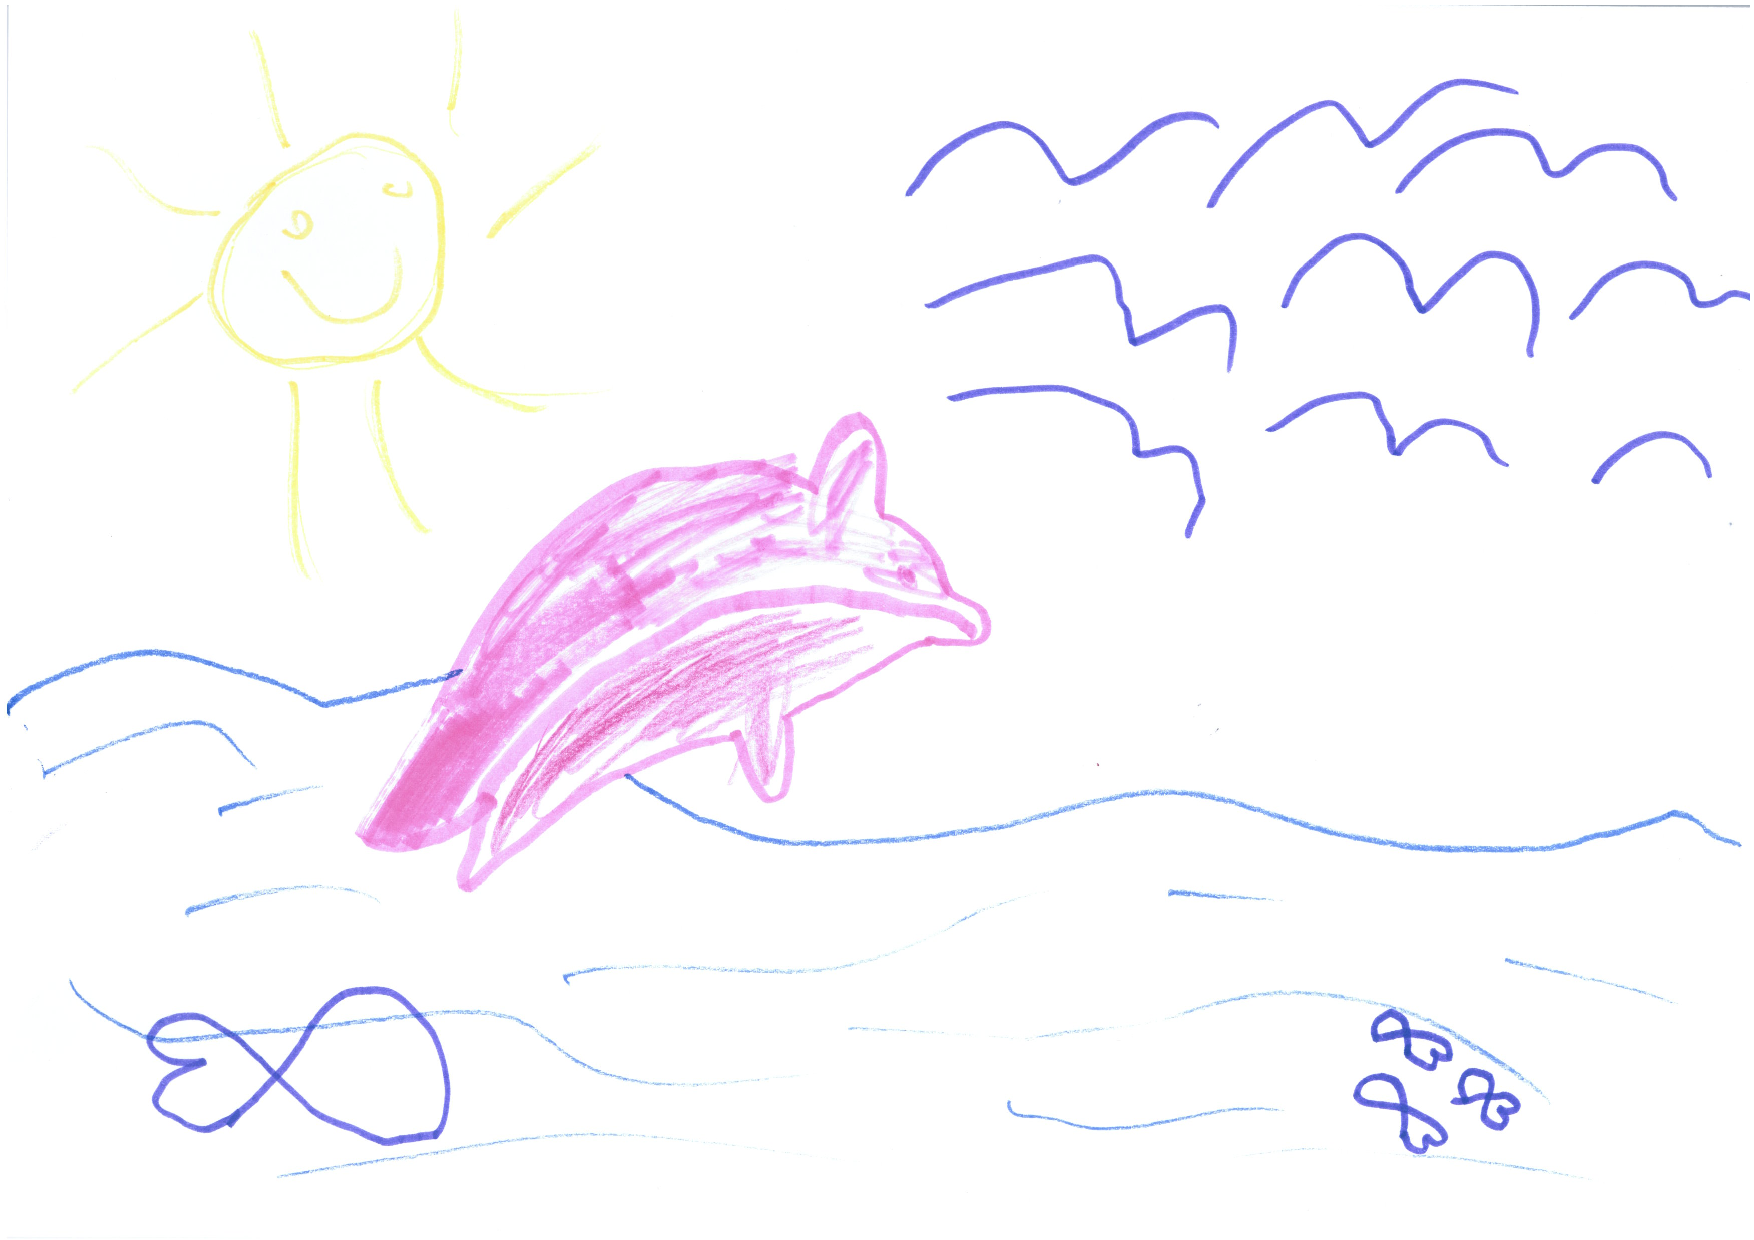
\includegraphics[width=.7\textwidth]{bilder/oma1.pdf}
\end{figure}
\medskip
\begin{mdframed}[style=mystyle]
Sie waren auf der Seite mit dem Delphinbild angekommen. Rosa war der und sprang gerade aus dem Wasser. Eine schöne Zeichnung, dachte Nina. Oma klappte das Buch zu und gab Nina einen Kuss auf die Stirn.

\enquote{Schlaf gut mein Engel.} sagte sie \enquote{Und morgen, gleich wenn Du aus dem Kindergarten zurück bist, lese ich Dir den Rest der Geschichte vor.} Selbstverständlich protestierte Nina. Wie kann man nur so gemein sein und aufhören, wenn es am spannendsten ist! Das war jetzt schon das zweite Mal an diesem Abend, dass sie sich vornehmen musste, es später, wenn sie selbst gross sein würde, besser zu machen. Aber noch bevor sie Oma eine Standpauke halten konnte, musste sie so fest gähnen, dass sie beschloss, auf lauten Protest zu verzichten. Dann eben morgen weiter.

Kater Fritz wurde noch aus dem Zimmer gescheucht, die Tür blieb einen Spalt offen und dann schlief Nina sofort ein.

Am nächsten Morgen konnte es Nina kaum abwarten, wie die Geschichte wohl weiterging. Die arme Rosa! Wie sie wohl wieder aus der Höhle kommen würde? Nina kontrollierte nochmals, dass das Buch auch so lag, dass Oma es gleich nehmen konnte, wenn sie zurück vom Kindergarten kam. Sie hatte so lange bei Mama gequängelt, bis diese versprochen hatte, dass es das Mittag erst gibt, wenn die Geschichte zu Ende erzählt war.

Endlich war es weit. Ohne wie sonst auf ihre Freundinnen zu warten, rannte Nina nach Hause. Oma sass schon lachend auf der Couch und meinte, Nina solle das Buch holen, es könne gleich los gehen.

Aber das Buch war nicht mehr da! Weg!

\enquote{Maaaaamaaaa, Maaaaaaaaamaaaaa! Wo hast du das Delphin-Buch hingelegt?} Nina war ausser sich. Mama kam die Treppe hinauf.

\enquote{Ich hab dein Buch nicht, Schatz. Wo hast du es denn hingelegt?} Auf so eine Frage antwortete Nina gar nicht erst. Als ob sie da nicht als allererstes gesucht hätte. Verzweifelt riss sie alle Bücher aus dem Büchergestell, aber das Delphin-Buch war nicht dabei.

Nina verzog sich in ihr Bett und schmollte. Mama versuchte zu trösten und versprach, das Buch zu suchen. Alle halfen mit und stellten die Wohnung auf den Kopf. Sogar die Möbel wurden verschoben, um nachzusehen, ob das Buch nicht irgendwo dahinter gefallen war. Aber es blieb verschwunden.  Endlich hatte Mama eine Erklärung. Fritz! Es konnte nur Kater Fritz gewesen sein. Wie ein Pfeil schoss Nina die Treppe herunter und schimpfte auf Fritz ein. Der aber gähnte nur und wollte gekrault werden. Wirklich böse konnte Nina ihm ja nicht sein, der wollte ja auch nur spielen.

So ging es den ganzen Nachmittag. Nina wollte doch unbedingt wissen, wie es bei Rosa und ihren Freunden weitergeht. Aber es war nichts zu machen. Am Abend, als es wieder Schlafenszeit war, streichelte Oma Nina über den Kopf und sagte:

\enquote{Manchmal braucht man gar keine Bücher, um Geschichten zu erzählen. Es ist ja nur das Buch weg, aber die Geschichte ist noch da. Du machst jetzt die Augen zu und konzentrierst dich ganz fest auf Rosa. Du musst ganz sehr an sie denken und dann wirst du schon sehen.}

Um wenigsten etwas von einem Delphin zu haben, nahm Nina ihren Spielzeugdelphin und legte ihn in ihren Spielzeugkoffer. Im Spielzeugkoffer waren immer die Lieblingsspielsachen von Nina, müsst ihr wissen. Und den Koffer stellte sie sich vor dem Schlafen immer ins Bett ans Fussende, damit all die wichtigen Dinge ganz nah bei ihr waren.

Wieder bekam Nina einen Kuss, zog die Decke über den Kopf und dachte an Rosa. Sie erzählte sich nochmals selbst die Geschichte, soweit sie sich an gestern Abend erinnern konnte und legte ihren Kopf gegen den Koffer\dots
\end{mdframed}\medskip

Plötzlich war auch Nina in der Höhle unter dem Meer. Sie hatte den Koffer mit ihren Lieblingsspielsachen unter dem Arm und sass auf einem Stein der aus dem Wasser ragte. Genau Rosa bemerkte auch sie als erstes diese Stille. Und das Licht von oben. Es war nicht zu erkennen, wo es herkam, aber es musste eine Höhle unter einer Insel sein überlegte Nina, denn sonst würde ja Wasser herein gelaufen kommen.

Nina hatte keine Angst. Sie wusste, dass es nur ein Traum war und ihr nichts passieren konnte. Wenn man träumt musste man nur ganz laut {\it Gefälligst aufwachen!} schreien, dann war der Traum sofort vorbei. Zur Sicherheit kniff sie sich in den Arm. Den Trick hatte ihr mal ihre Cousine gezeigt. Die war schon drei Jahre älter und wusste daher alles. Wenn man sich kneift und etwas spürt, ist alles in Ordnung. Wenn man nichts spürt, träumt man gerade, hatte die erklärt. Und tatsächlich, Nina spürte nichts.

\enquote{Haaallllooo} rief Nina ganz laut.

\enquote{--lo, --lo, --lo} schalte es von allen Seiten zurück. Ein Echo in einem Traum? Sehr merkwürdig. Oder gab es so etwas? Nina war unschlüssig. Doch, vermutlich gibt es so etwas, entschied sie. Aber in einem Traum darüber nachdenken, ob man träumt und woran man eigentlich merkt, dass man träumt, das gab es ja eigentlich nicht. Na jedenfalls hatte es Nina noch nie erlebt. Du vielleicht?

Stopp! Denk jetzt nicht zu viel darüber nach, denn Nina sieht gerade, wie eins, zwei, drei, nein, fünf rosa Delphinköpfe aus dem Wasser lugen. Das Licht der Höhle glänzte auf ihren glatten Köpfen. 

\enquote{Ich bin Nina.} sagt Nina, weil sie gerade nicht weiss, was man sonst in dieser Situation tun können. Als die Delphine antworten und nicht einmal zu bemerken scheinen, dass sie mit einem Menschen reden, ist Nina beruhigt. Dann kann alles ja nur ein Traum sein! Weniger beruhigend ist dagegen, was die Delphine erzählen.

Rosa fängt an: \enquote{Da draussen schwimmt ein riesiger Hai. Der hat gesehen, dass wir hier in die Höhle geflüchtet sind und wartet jetzt auf uns.}

\enquote{Aber das ist noch nicht das Schlimmste!} ruft einer ihrer Freunde dazwischen. \enquote{Rosa ist verletzt und die Wunde hat sich entzündet.}

Rosa entscheidet, dass zuerst die Wunde behandelt werden muss. Wenn sie selbst sich verletzt hat, wird die Wunde erst gereinigt, dann sprüht ihr Papa immer aus einem kleinen Fläschchen etwas auf die Wunde und zum Schluss kommt ein Pflaster darauf. Das Fläschchen und das Pflaster holt Papa immer aus einem Schrank im Bad, der für sie verboten ist. 

\enquote{Das haben die Erwachsenen von ihren Regeln}, denkt Nina, \enquote{Jetzt kenne ich mich gar nicht aus!} Wenn sie zu Hause wäre, hätte sie Pflaster. Sie verarztet immer ihre Puppen und dafür hat sie einmal ein grosses Stück bekommen, das bewahrt sie immer in ihrem Spielzeugkoffer auf.

\enquote{Aber natürlich!} ruft sie, den Koffer hat sie ja glücklicherweise bei sich! Zunächst einmal nachsehen, was alles gerade in dem Koffer war. Ein Nuschi, eine Schnur, ein Bild von einem sehr süssen kleinen Hund, natürlich der Delphin und tatsächlich! Pflaster! 

Rosa musste ihre verletzte Flosse auf den Stein legen. Gar nicht so leicht. Mit dem Nuschi tupfte Nina die Wunde ab. Aber das Spray fehlte, das war nicht zu leugnen. Nina wusste nicht genau, ob das wichtig war. Sie betrachtete noch einmal die Dinge in ihrem Koffer. Beim Bild des kleinen Hundes kam ihr eine Idee. Sie hatte schon einmal gesehen, dass ein Hund auf eine Scherbe getreten war und sich dann die Wunde abgeleckt hat. Das war es!

\enquote{Ihr müsst jetzt die Wunde ablecken!} rief sie den Freunden von Rosa zu. Die wussten zwar nicht so genau wieso, glaubten ihr aber einfachen und taten wie gesagt. Als sie fertig waren klebte Nina ein Pflaster über die Wunde.

\enquote{So!} sagte sie, \enquote{Das hätten wir geschafft.} Und tatsächlich konnte Rosa bestätigen, dass die Wunde eigentlich nur noch halb so weh tat. Jetzt blieb nur noch der Hai. Inzwischen war Fridolin zurück gekommen und brachte Fische. Nina probierte lieber nicht. Der rohe Fisch, noch mit Haut, war wohl eher nichts für sie.

\enquote{Ja, der Hai ist noch da.} musste Fridolin bestätigen. \enquote{Und ich befürchte er ist mittlerweile vor lauter Hunger noch wilder als das letzte Mal. Er hat hier die ganze Zeit gewartet. Und wenn wir nicht bald etwas unternehmen, werden noch andere Haie angelockt und dann schaffe es selbst ich nicht mehr aus der Höhle.} Verzweiflung war in seiner Stimme.

Nach dem Essen fingen alle sehr angestrengt an nachzudenken. Niemand wusste etwas Gescheites. Wieder war es Nina, die die rettende Idee hatte. Sie flüsterte Fridolin etwas ins Ohr. Dann öffnete sie wieder den Spielzeugkoffer und fing an zu basteln. 

Nach einer halben Stunde ging es los. Zuerst schwamm Fridolin aus der Höhle. Dann folgten die fünf Freunde, ein Delphin nach dem anderen. Sie huschten nach links und rechts und oben und unten, nachdem sie aus dem Höhleneingang heraus geschwommen kamen. Aber auch der Hai war da. Und er bemerkte die Delphine sofort.

Da hat er schon den ersten ins Visier genommen. Er stürmte auf den Delphin los. Schnell war er ganz dicht hinter ihm, seine Nase berührte schon die Schwanzflosse, riss sein ungeheures Maul auf und rrrrrrrrrammms, biss er zu! Aber was war das? Mit einem gewaltigen Knall krachte er gegen die Felswand. Der Hai hatte den Delphin verpasst. Seine Nase blutete.

Aber so etwas macht einen richtigen Hai nur noch wilder. Er sah sich um. Diesmal ruhiger. Der Hunger hatte ihm den Kopf vernebelt, das merkte er jetzt. Jetzt heisst es wieder den klaren Kopf eines guten Jägers zu haben. Schon wieder hat er einen Delphin entdeckt, und dort war auch gleich noch einer. Und da schon wieder. Und dort. Und da noch mehr, dutzende, hunderte. Der Hai war völlig verwirrt. Er überlegte, ob es der Stoss liegen könne, dass er nicht mehr richtig sehen könne?

Jetzt bemerkte er auch Fridolin. An die Schildkröte konnte er sich gut erinnern, die hatte ihn so böse von der Seite erwischt. Aber was zog die hinter sich her? Eine Schnur, an die ein Delphin gebunden war? Mit zwei starken Stössen war er bei dem Delphin an der Schnur und ohne zu zögern biss er zu.

Er klebriger Geschmack machte sich in seinem Mund breit. Den Geschmack kannte er. Plastik. So etwas schmeissen die Menschen manchmal aus ihren Schiffen ins Wasser. Das hatte er schon einmal probiert, ungeniessbar und danach bekommt man Bauchschmerzen. Hatte ihm jemand einen Streich gespielt? Der Hai schwamm wütend im Kreis. Und überhaupt überlegte er dabei, seit wann sind denn Delphine rosa? So etwas gibt es ja nur im Amazonas, aber doch nicht hier. Die sind bestimmt auch nur aus Plastik, war letztlich überzeugt.  Und weil er sowieso lieber mit seiner blutigen Nase nach Hause wollte als möglicherweise nur Plastik zu jagen, schwamm er davon.

Rosa hatte das alles vom Eingang der Höhle aus beobachtet und musste Nina haargenau erklären, was passiert war. Genau das war ja Ninas Plan gewesen. Frisolin sollte den Spielzeugdelphin aus dem Koffer hinter sich herziehen. Die Kristalle des Felsens würden diesen immer wieder spiegeln. Es musste den Hai einfach verwirren, wenn er so viele Delphine sieht. Eigentlich war es Ninas Plan gewesen, dass Rosa und ihre Freunde genau in dem Augenblick die Höhle verlassen, Als der Hai das erste Mal gegen die Wand kracht. Dann hatte sich aber doch keiner der fünf Freunde aus der Höhle getraut, als der Hai so wild geworden war.

Aber so war der Hai ja von alleine weg geschwommen. Sie konnten jetzt beruhigt nach Hause schwimmen. Fridolin vorne weg und die Delphine hinterher. Aber erst mussten sie sich von Nina verabschieden, denn die konnte natürlich nicht tauchen und schwimmen wie ein Delphin. 

Die Delphine folgten der Schildkröte hinaus aus der Höhle und los ging die Heimreise. Es dauerte nicht lange, da schmeckte das Wasser schon nicht mehr so salzig und schon bald so, wie es unsere fünf Freunde gewohnt waren. Die ersten Bäume tauchten wieder auf, sie waren beim Festland angekommen. Jetzt verabschiedete sich auch Fridolin. Alle durften einer nach dem anderen nochmals über Fridolin drüber springen, so macht man das als Delphin, wenn man zeigen will, dass man jemanden gern hat. Die fünf rosa Delphine mussten jetzt nur noch flussaufwärts schwimmen. Nach ein paar Tagen, kamen sie erschöpft in ihrem Nebenarm an.

Ihr könnt euch vorstellen, was das für eine Party geworden ist! Drei Tage und viel mehr Nächte feierten alle Tiere des Nebenarms. Und selbst das Faultier liess sich nachdem er ein paar überreife Früchte gegessen hatte hinreissen, einen Cha Cha Cha zu tanzen. Das war sicher der Höhepunkt des Festes. Die fünf Freunde aber mussten als erstes einmal ganz in Ruhe schlafen. Ihre Väter und Mütter kamen zu ihnen ans Bett. Lobten sie und sagten, sie wären jetzt grosse Delphine und gaben ihnen einen Kuss. Die fünf Freunde schlossen jeder in seiner Schlafecke die Augen und träumten von Tina und ihrem Spielzeugkoffer.

\medskip
\begin{mdframed}[style=mystyle]
Der Wecker klingelte. Nina wachte in ihrem Bett auf. Ungläubig sah sie sich in alle Richtungen um. Jetzt war klar, dass es doch ein Traum gewesen sein musste. Oma spienzelt zur Tür herein.

\enquote{Na, schon wach?} Nina musste sich erst einmal richtig strecken und auf die andere Seite drehen, bevor sie antworten konnte. Aber das war normal, das war jeden Tag so.

\enquote{Ich habe von Rosa geträumt.} schaffte sie dann aber doch zu sagen. Oma lächelte. Dann erzählte Nina genau, was sie geträumt hatte. Und als sie an die Stelle kam, wo sie ihren Spielzeugdelphin an die Schnur geknotet hatte, nahm sie ihren Spielzeugkoffer. Der lag geöffnet neben dem Bett, er war wohl nachts runtergefallen. Es fehlte nichts, alles war noch da. Nur von ihrem Delphin fehlte ein Stück von der Schwanzflosse. Nina blieb beinahe das Herz stehen. Gestern war das doch noch nicht so gewesen? Sollte doch der Hai\dots?

Aber in dem Moment kam Kater Fritz durch die Tür geschlichen und da wusste Nina, dass es bestimmt kein Hai gewesen war, der ihrem Spielzeug in den Schwanz gebissen hat. 
\end{mdframed}\medskip
